\documentclass{article}
\usepackage{ctex}
\newcommand{\prb}{\times 10^5~\mathrm{kPa}}
\newcommand{\pre}{~\mathrm{kPa}}
\newcommand{\vol}{~\mathrm{mm^3}}
\newcommand{\are}{~\mathrm{mm^2}}
\newcommand{\len}{~\mathrm{mm}}
\newcommand{\tim}{~\mathrm{ms}}
\newcommand{\vel}{~\mathrm{ms^{-1}}}
\newcommand{\mas}{~\mathrm{mg}}
\newcommand{\den}{~\mathrm{mg~mm^{-3}}}

\begin{document}
\section{摘要}
	本文中我们先给出了每一题的基本分析和思路,再给出了它们的具体解题过程。

	对于问题一,我们假定燃油在油管内压强均匀,高压泵的流量符合题中注2所给公式。我们预先根据题目中给的弹性模量和压强的关系,用梯形法数值积分得到了在离散点上燃油密度和压强的对应关系,同时在后面程序使用时通过线性内插得到完整函数关系。我们先通过稳压近似方法,利用长时间内燃油支出平衡给出单向阀开启时长的理论值;再通过将时间离散化,用数值模拟的方法给出压强精确演化规律,并对两种方法的结果进行了交叉验证。
	
	对于问题二,我们建立了一个考虑了油泵和喷油器工作原理的油管演化模型。我们预先利用凸轮的外轮廓形状计算了在给定转角下柱塞的抬升高度。再将燃油在喷油器内的行为近似为了两次扩散过程,并利用已知的针阀升程的变化,通过割线法求解了给定时间和油管压强下的喷油器流量。最后我们将油泵、油管和喷油器三个部件组合到一起,完成系统的模拟演化程序。我们定义关于目标压强的方均根偏差作为压强偏离的量度,得出了最优凸轮角速度为$\omega=0.0238\vel$。
	
	对于问题三,首先我们从上一问找出了压强波动的原因。联系实际情况给出了系统的可变量。我们先对减压阀可连续调节的情况,通过定性半定量分析得出最优的控制方案应满足的条件,再通过数值模拟和调参得到具体的控制方案,该方案能够将压强波动缩小接近100倍。然后又考虑了实际应用中可能对阀门控制有所限制,构造了另一种阀门操作频率很低的控制方案,能将压强波动缩小约4倍,并从理论上证明了在给定限制条件下该方案的最优性。
	
	在本文的最后,我们对上述建立的模型进行了评价,说明了它的合理性和可拓展性,同时指出了一些近似导致的模型的局限性。

	【关键词】	高压油管 数值模拟 稳压控制
\section{问题的表述与分析}
	\subsection{问题 3}
	\subsubsection{问题 3 的表述}
	在问题2的基础上,现在我们需要同时给两个喷嘴B和C供油。同时在D处安装一个单向减压阀。打开减压阀时高压油管内的燃油可以回流到外部低压油路中,使得高压油管内的压强减小。
	B和C两个喷嘴的喷油规律与问题2中相同;考虑到实际应用,喷嘴B和C能够人为变化的只有二者分别的第一次的喷油时间,而喷油频率为每秒10次保持不变。高压油泵的转速可以认为变化,但假设仍为匀速转动。
	D处单向减压阀也可以主动开启和关闭,但是由于题目并没有明确说明减压阀是否可以连续控制,在本题中我们将按以下两种情况进行分类讨论:
	\begin{enumerate}
		\item 单向减压阀可以随时开启和关闭,不受任何的限制
		\item 与问题1中单向阀类似,单向减压阀每次开启后需要至少10ms的关闭时间
	\end{enumerate}
	问题可以表述为:如何调整B和C喷嘴的喷油时间,凸轮的角速度,以及如何控制D处减压阀的开启和关闭,使得高压油管的波动值最小。
	\begin{figure}[!ht]
		\centering
		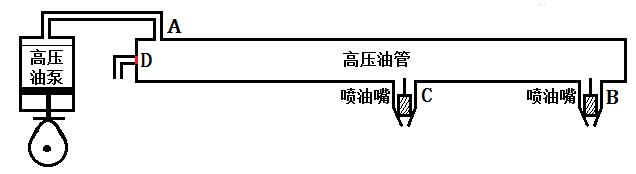
\includegraphics[scale = 1.1]{sketch3.jpg}
		\caption{系统 3 的示意图}
	\end{figure}
	\subsubsection{问题 3 的分析}
	理解此问题的关键在于找到压强波动的原因。由于具体分析需要用到问题2的结果,后文将有详细解读,在此不再赘述。
	
\section{模型的建立与求解}
	\subsection{问题3-减压阀连续可调情况}
	\subsubsection{定性分析}
	我们按照以下的逻辑顺序进行分析:
		\begin{enumerate}
		\item 
		在问题2中我们看到,压力波动是由于喷油和泵油的时间不一致造成的。如果能在喷油的同时泵油,就能使得$P-t$图曲线斜率大小降低,压力波动变小。
		\item 
		首先我们定义每毫秒高压油泵泵入的油量随时间的关系为“泵油曲线”,每毫秒通过B或C喷嘴喷出的煤油质量随时间的变化关系称为“喷油曲线”,而将每毫秒高压油泵供给的煤油减去减压阀释放的煤油随时间的变化曲线称为“供油曲线”。
		\item 
		显然,我们的目的是使供油曲线和喷油曲线尽量重合,这样油管内总油量离标准值的差就越小,压力波动就越小。最理想的情况,供油曲线和喷油曲线完全重合,此时油管内压强不变。
		\item
		通过减压阀的连续控制,可以利用开启减压阀来抵消油泵的供油,从而将供油曲线向下调整。例如在喷嘴没有喷油的情况下,油泵却在泵油,此时若管内压强大于$1\prb$则开启减压阀,反之则关闭减压阀,可以保证压强准确维持在标准值附近(即供油曲线向下调整至0)。\\当然,测量压强并实时反馈在应用中做不到,我们只是通过这种手段寻找控制策略;而一旦找到策略,应用时只需按照时间开关减压阀即可,不再需要测量和反馈。
		\item 
		上述调节成立的条件是减压阀的泄流速度大于油泵的供油速度。当油泵凸轮角速度很快时泵油流量可能会非常大,以至于打开减压阀时油管内压力仍然上升,调节功能失效。因此油泵角速度有上限值。
		\item 
		为了长时间的精确调节,油泵的周期和喷油周期应当是简单整数比的关系。喷油的速率较大且比较恒定,为了使供油曲线贴近喷油曲线,油泵的周期应该较小。合理的假设是油泵周期为喷油周期的整数分之一倍。\\
		为了使油泵角速度较大,以及对称性考虑,B和C两油泵应该交替喷油,等效于$\tau_0=50\tim$的喷油周期
		\item
		综上,以下示意图分别为:图A-泵油曲线,图B-供油曲线,图C-喷油曲线(这里画的是N=3的情况,但实际上N也是可变的)\\
		
		(此处应有三张示意图ABC)\\
		
		通过调节减压阀,可将供油曲线从图A调节为图B模样,使得图B贴近图C。为了支出平衡要求阴影部分面积相等\\
		油泵角速度为$\omega=\frac{2\pi{}N}{\tau_0}$,N为整数,$\tau_0=50\tim$
	\end{enumerate}
	\subsubsection{精确数值模拟}
		除了喷油周期改变为原来一半外,相较于问题2中的程序,此题中数值模拟程序的改变主要体现在煤油质量更新的部分。\\\\
		定义dm为假设此刻开启减压阀门的情况下,dt时间内从减压阀流出的油量,则在图B的阴影部分之外:
		\begin{enumerate}
		\item 
		若压力低于标准值,$m_2 \leftarrow m_2 + Q_A \times \rho_1 \times dt - Q_B \times \rho_2 \times dt$
		\item 
		若压力高于标准值,$m_2 \leftarrow m_2 + Q_A \times \rho_1 \times dt - Q_B \times \rho_2 \times dt - dm$
		\end{enumerate}
		而图B阴影部分之内仍然不变(减压阀保持关闭)\\\\
		图B的阴影部分较图C的阴影更矮胖一点,N越大图B的阴影越高越尖,也就更贴近喷油曲线。然而模拟发现$N\ge 4$时减压阀泄流速度有时小于泵油速度,调节功能失效。因此可以肯定N=3为最优方案。\\\\
		经过手动调参(喷油起始时间)得到最优方案时结果如下:\\
		
		(此处应有P-t图1)\\
		
		由于此时$Q_A$与$Q_B$很接近,供油和喷油速率的差较小$(\frac{dm_A}{dm_B}\approx1.08)$,压强的波动很小,即使峰值也只有约$70\pre$。方均根更是低达$D=11\pre$,大约是优化前的百分之一。调控性能非常优秀!\\
		
		综上,最优控制方案为:
		\begin{itemize}
			\item 高压泵凸轮转动周期为 $\tau_A=\frac{50}{3}\tim$
			\item B、C喷嘴等间隔交替喷油(等效喷油周期$50\tim$)
			\item 喷嘴和凸轮转动周期的开始时间差(即相位差)为$2.0\tim$
			\item 
			减压阀工作的时间为每个$50\tim$周期内(初始时刻油泵柱塞在最低点)的$1.95\tim$之前和$4.3\tim$之后。在工作时间外减压阀关闭,在工作时间内(此时喷嘴不会喷油)减压阀负责抵消油泵的进油,将油管内压力稳定在标准值$1\prb$。
		\end{itemize}
	
	\subsection{问题3-减压阀调节受限情况}
	\subsubsection{定性半定量分析}
		现在我们假设由于实际应用时的限制,减压阀每次开启后至少要关闭$10\tim$的时间。此时分析问题的总体思路与之前一样,即欲使供油曲线与喷油曲线贴合,但由于条件限制具体的策略也会有改变。\\
		由于系统有$100\tim$的周期性,设$\omega=\frac{2\pi{}N}{\tau_0}$\\
		其中$\tau_0=100\tim$,N为整数\\
		
		由于油管压力变化不大,首先取油管压强为恒为$1\prb$做估算,以定性半定量地得出一些有意义的结论。利用这个近似的数值模拟计算可快速得到:
		\begin{enumerate}
			\item
			当$N=2$时,泵油时$dt(=0.01\tim)$时间内高压泵泵入的油量典型大小约为$dm_A=0.05\mas$,泵油的持续时间约为$t_A=18\tim$
			\item
			若打开减压阀,dt时间内减压阀流出的油量为$dm_D=0.170\mas$
			\item 
			喷嘴dt时间内喷出煤油质量为$dm_B=0.150\mas$
			\item 
			由$E=\frac{\Delta{P}}{\Delta{\rho}/\rho}=\frac{dP}{dm/m_2}$。得$\frac{dP}{dt}=\frac{E}{m}\frac{dm}{dt}$,取E为$1\prb$时的估算可得油泵提供的油管内压强增加率约为$(\frac{dP}{dt})_A=325~\mathrm{kPa/ms}$,\\减压阀提供的压强减少率约为$(\frac{dP}{dt})_D=-1107~\mathrm{kPa/ms}$,\\喷嘴提供的压强减少率为$(\frac{dP}{dt})_B=-975~\mathrm{kPa/ms}$
			\item 
			凸轮转一圈泵油量约为$76\mas$,喷嘴每次喷油量约为$29\mas$,因此若一个周期内同时有油泵泵油和喷嘴喷油,剩余$47\mas$的油需要通过减压阀释放。减压阀总开启时间由此算出为$2.8\tim$
			\item 
			若N=3,至少有一个凸轮旋转周期内没有喷嘴喷油,则$t_A=18\tim$的时间长度内至少有$7.5\tim$是减压阀关闭(减压阀不能连续开启,最好的状态就是在$t_A=18\tim$的中间开启减压阀,减压阀总开启时间为$2.8\tim$),同时油泵在泵油的状态。根据泵油速度计算,这$7.5\tim$中不可避免增加的油压约为$1500\pre$。当N更大时这个压强增加值会更大。为了让油压波动较小,必有$N<3$
			\item 
			另一方面,为了让泵油能更多抵消部分喷油导致的压降,N越大越好。
			\item
			当N=2时,在喷嘴完全开启的$2\tim$中,即使油泵也处于开启状态且减压阀关闭,压强也会下降约$1300\pre$。总的压强极差不可能小于这个值。也就是说,我们只要构造了一个压强的极差在$1300\pre$左右的控制方案,它就是最佳的方案了
		\end{enumerate}
	\subsubsection{方案构造}
		根据上一节分析,最优方案为N=2时压强极差在$1300\pre$左右,这个限制是因为喷嘴喷油过快导致,无法避免。下面我们就尝试构造这样一种方案。

		首先因为N=2,且每个凸轮轴期内都要有喷嘴喷油,所以B、C两喷嘴应交替喷油。于是可以等效成一个$\tau_0=50\tim$的喷嘴,凸轮周期和喷嘴周期相同。我们只需要完成一个周期内的构造,并且让此周期结束时和开始时的压强相等即可。
		
		压力变化等价于油量变化。减压阀每次放油量不应超过喷嘴每次喷油量$29\mas$,这样压降才不会超过$1700\pre$。由于$29\times 2<76<29\times 3$,应该有一次喷嘴喷油和两次减压阀放油。考虑到减压阀开启有限制,喷嘴喷油应在两次放油之间。通过上述分析可以得到以下控制思路:\\
		
		(此处应该有示意图2)\\
		
		上图中,$t_A^+$开始高压油泵中有油泵出,泵油过程直到$t_A^-$才停止。在大部分时间油管内由于高压油泵泵油而压强增大;而在$t_{D1}$附近减压阀开启压强下降,$t_B$附近喷嘴喷油导致压强下降,$t_{D2}$附近减压阀第二次开启。
		
		$t_B$附近$1300\pre$的压降无可避免,我们要做的是调节$t_{D1}$和$t_{D2}$及减压阀开启时间使得压强的波动范围在这个限度以内,并且最终管内压强能回到标准压强。
	
	\subsubsection{精确数值模拟}
		我们沿用之前连续可调情况下的模拟程序,但是由于减压阀开启限制需要做一些调整:
		\begin{enumerate}
			\item 
			定义布尔变量D\_lock记录减压阀是否处于锁定的不可开启状态,并用D\_remain\_time记录锁定的剩余时间。只有在减压阀未锁定时可以对其进行操作。
			\item 
			每当减压阀被关闭时,进入$10\tim$的锁定时间
			\item 
			更新油管总油量$m_2$的代码区域需要做出较大改变。在减压阀锁定时直接按照无减压阀的情况更新$m_2$。而在减压阀未锁定时需要根据此刻的时间和系统状态判断在示意图中哪个部分,以给减压阀正确的开关指令。
		\end{enumerate}
		最终程序给出的模拟结果如下:\\
		
		(此处应该有P-t图2)\\
		
		最终结果压强波动时偏离标准值的峰值为$630\pre$,即极差约为$1280\pre$,符合最优解的要求。计算得到此策略下方均根偏差为$D=226\pre$,小于优化前的四分之一,效果显著!\\
		
		综上,我们的最终控制方案为:
		\begin{itemize}
			\item 高压泵凸轮转动周期为 $\tau_A=50\tim$,B、C喷嘴等间隔交替喷油
			\item 喷嘴和凸轮转动周期的开始时间差(即相位差)为$10.35\tim$
			\item 减压阀开启的时间为每个$50\tim$周期内(初始时刻油泵柱塞在最低点)的
			[$4.84\tim$, $6.29\tim$]和[$17.43\tim$, $18.75\tim$]
		\end{itemize}
		
\section{模型的评价} % 优缺点、改进空间和范围
	\subsection{问题1}
		该题中的模型所做的假设是管内压强是均匀的,在单向阀处煤油的流量根据注2计算。不考虑煤油的粘滞、涡流等复杂液体行为,也没有考虑煤油如何在油管内从A处流动至B处。由于条件本身也是抽象化的,省略了很多细节,因此模型也简洁而清晰。
		
		当然也正是因为其简洁性,没有太多实际应用的价值。
	\subsection{问题2}
		在问题2中,我们将问题1的高压泵和喷嘴具象化了,考虑了他们的工作原理。
		这个模型同样认为所有封闭腔内的压强是均匀的,煤油是静止的,忽略了煤油的复杂流体性质。还有一个重要的假设是把喷嘴内的流动看做是连续两次扩散过程。
		
		然而实际上喷嘴处煤油的流动是非常复杂的,较精确的计算要使用混合多相流模型附加空穴模型,本题这里的近似较为粗糙,这也是此模型最大的缺陷。
		
		但本模型的优点在于可修改性强,整个程序的核心物理量是管内煤油的质量$m_B$,而油泵和喷嘴对$m_B$的全部影响都体现为油管压强$P_2$和时间t的一个二元函数,这些函数互不干扰。因此后续改进可以是精确计算喷嘴的流量模型,然后修改主程序中对应的函数即可,其它部分不受影响。
		
		本模型另一个优点是可拓展性强。比如说加一个喷嘴或者加一个阀门,都只要更新$m_B$时加两个函数值即可,这也为问题3提供了方便。
	\subsection{问题3}
		问题3的模型主要是通过减压阀的控制,实现了更加稳定的油管压力。
		该模型联系了实际。喷嘴是给发动机供油的,而发动机转速在短时间内一般不会剧烈改变,因此模型假定了喷嘴的喷油周期是恒定的。凸轮的角速度也很难快速地精确控制,因此假定了凸轮是匀速旋转。
		
		模型最终实现了非常好的稳压效果。若能连续调控减压阀,压强变化量几乎可以忽略。若考虑可能的实际情况,在减压阀调控受限时,通过一个周期内给定时间段仅开启两次减压阀也能实现不俗的效果。并且前文也证明了在这些假定下上述调控方案是最优的。
		
		从实际情况来看,更好地实现稳压需要更加精细的模型,例如要考虑针阀开启或关闭瞬间由于液体流动行为突然变化导致的压力波动。而实际情况中可能出现的影响压力的这些因素由于涉及到流体性质在本模型中无法计算。
		
		作为稳压装置,本油管的改进可以通过增加一个减压阀,允许更大的凸轮转速。也可以改变凸轮的形状,使油泵的泵油在一个周期内更加集中。
\end{document} 